\chapter{Probabilità}
Il calcolo delle probabilità è una teoria della matematica che permette di descrivere e studiare \underline{Fenomeni Aleatori}.
\\Un \textbf{Fenomeno Aleaotrio} (o casuale) é un fenomeno il cui esito \emph{non è prevedibile con certezza} a priori.
\section{Assiomi della Probabilità}
La probabilitá si basa sullo studio di \textbf{Esperimenti Aleatori}, ovvero esperimenti il cui risultto non è prevedibile con certezza.
Per poter studiare gli eseprimenti aleatori bisogna poterli descrivere matematicamente. 
La loro descrizione matematica si articola in tre passi:
\begin{enumerate}
    \item \textbf{Spazio campionario} (o spazio degli esiti)
    \\ $\to$ Insieme $\Omega$ che contiene tutti i possibili esiti dell'esperimento 
    \\ \small{es. Tiro un dado a sei facce $\Omega = {1, 2, 3, 4, 5, 6}$}
    \item \textbf{Eventi}
    \\ $\to$ I sottinsiemi dello spazio campionario $A \subseteq \Omega$ che riassumono affermazioni sull'esito dell'esperimento aleatorio.
    \\ \small{es. Tiro un dado a sei facce: esce un numero pari $A = {2, 4, 6}$}
    \item \textbf{Probabilità}
    \\ $\to$ Regola che assegna, in modo coerente, a ogni evento $A \subseteq \Omega$ un "\textbf{grado di fiducia}" $P(A)$, tra 0 e 1, che attribuiamo al verificarsi di A.
\end{enumerate}
Matematicamente la \textbf{Probabilità} é una funzione $P:\rho(\Omega) \to [0,1]$ che soddisfa opportune proprietá.
In questo caso $\rho(\Omega)$ sono tutti i sottoinsiemi di $\Omega$.

\subsection*{Operazioni insiemistiche e Logiche}
Nella definizione degli eventi, che sono concetti logici tradotti in concetti insiemistici, ci sono dei parallelismi tra le operazioni logiche e quelle insiemistiche:
\begin{itemize}
    \item Unione $A\cup B$ $\longleftrightarrow$ Si verifica $A$ o $B$ o entrambi.
    \item Intersezione $A \cap B$ $\longleftrightarrow$ Si verificano $A$ e $B$.
    \item Complementare $A^c$ $\longleftrightarrow$ Non si verifica $A$.
\end{itemize}
Ci sono poi anche due interessanti proprietá dei complementari:
\begin{itemize}
    \item $(A^c)^c = A$ (doppia negazione)
    \item Leggi di Demorgan: $(A \cup B)^c = A^c \cap B^c$ e $(A \cap B)^c = A^c \cup B^c$
\end{itemize}

\subsection{Interpretazioni di $P(A)$}
Che cosa significa grado di fiducia? cosé $P(A)$?
\\Esistono due diverse interpretazioni sul grado di fiducia, entrambe equamente valide:
\paragraph{Interpretazione Soggettivista} In questa interpretazione $P(A)$ é il prezzo equo di una scommessa che paga 1 se si 
verifica $A$ e 0 altrimenti.
\paragraph{Intrepretazione Frequentista} In questa interpretazione invece $P(A)$ è la frazione asintotica di volte in cui si verifica $A$ ripetendo l'esperimento.

\paragraph*{}Quale scelgo? Entrambe queste interpretazioni sono valide, quindi si puó scegliere quella che si vuole.
Tutte e due queste interpretazioni peró devono soddisfare le due Proprietà di Base.

\section{Proprietà di base} 
Ogni interpretazione probabilistica deve rispettare queste due proprietà fondamentali:
\begin{enumerate}
    \item $P(\Omega) = 1$, ovvero la probabilitá dello spazio campionario deve essere 1 (massima).
    \item Se A e B sono eventi disgiunti, cioè $A \cap B \neq \emptyset$, allora deve valere che $P (A \cup B) = P(A) + P(B)$
\end{enumerate}
Da queste proprietá si deriva la Definizione dell'approccio moderno alla probabilitá, definito da Kolmogorov nel 1933:
\definizione{
    Sia $\Omega$ un insieme (spazio campionario).
    Si dice \textbf{Probabilità} qualsiasi funzione $P:\rho(\Omega) \to [0,1]$ che soddisfa:
    \begin{enumerate}
        \item $P(\Omega)= 1$
        \item Se $A\cap B = \emptyset \implies P(A \cup B) = P(A) + P(B)$.
    \end{enumerate}
    La coppia $(\Omega, P)$ é detta \textbf{Spazio di Probabilità}
}

\osservazione{Se $\Omega$ è più che numerabile (ad esempio $\R$ o $[0,\infty]$)
Una probabilità può essere definita solo per una classe $A\subseteq P(\Omega)$ di elementi.
}

\paragraph{Proprietà di Base}
Fissiamo uno spazio di probabilità $(\Omega, P)$ e consideriamo le proprietà 1 e 2 della definizione.
Da queste proprietà si deducono le seguenti altre proprietà.
\\Fissiamo la prpoposizione $P(\emptyset) = 0$:
\begin{itemize}
    \item \textbf{Regola del complementare} 
    $$P(A^c) = 1 - P(A) \;\;\;\forall A$$
    \item \textbf{Regola della addizione di probabilità} 
    $$\to P(A \cup B) = P(A) + P(B) - P(A \cap B)  \;\;\;\forall A,B$$
    \\ Vale anche $A \cap B \neq \emptyset$
    \item \textbf{Monotonia}
    \begin{center}
        Se $A \subseteq B$ allora $P(A) <= P(B)$
    \end{center}
\end{itemize}
\paragraph{Analogia} c'è un analogia tra probabilità e area
\begin{center}
    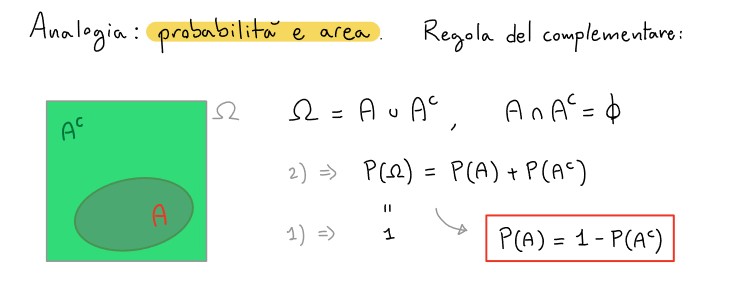
\includegraphics[width=120mm,scale=0.5]{analogia_prob_area.png}
\end{center}

\paragraph*{Insiemi disgiunti Multipli}
Dalla seconda proprietà (Se $A\cap B = \emptyset \implies P(A \cup B) = P(A) + P(B)$) segue che:
\\Se $A_1,A_2,...,A_k$ sono insimi disgiunti, per cui $A_m \cap A_n = \emptyset, m\neq n$, allora varrà che:
\[ P(A_1 \cup A_2 \cup ... \cup A_k)= P(A_1) + P(A_2) + ... + P(A_k)\]
Per sviluppare la \textbf{Teoria Matematica} però è richiesto qualcosa in più.
%Non la riporto per mancanza di tempo, pagina 1 appunti lezione 3


\subsection{Spazio di Probabilità Uniforme}
Introduciamo ora il concetto di Spazio di Probabilità uniforme:
\definizione{
    Indichiamo con $|A|$ la Cardinalità, ovvero il numero di elementi, dell'insieme $A$.
    \\La \textbf{Probabilità Uniforme} su un insieme finito $\Omega$ è:
    \[ P(A):= \frac{|A|}{|\Omega|}=\frac{\text{Casi Favorevoli}}{\text{Casi Possibili}} \text{ per ogni }A \subseteq \Omega\]
    In particolare, per un singolo elemento varrà:
    \[P({w}) = \frac{1}{\Omega} = \frac{1}{n} \text{ per ogni } \in \Omega\]
    }
La probabilità uniforme è l'unica che mi da \textbf{la stessa probabilità per ogni elemento}.
\nb{La P.Uniforme non è l'unico tipo di probabilità esistente}
Questo è il modello appropriato per descrivere esperimenti aleatori i cui esiti siano tutti \textbf{equiprobabili}.
Quando scegliamo casualmente una persona/oggetto in un insieme finito senza ulteriori specifiche, si sottintende che la scelta è effettuata in modo uniforme.
Affinchè la probabilità uniforme sia ben definita, lo spazio campionario $\Omega$
deve essere finito (se così non fosse la probabilità uniforme su $\Omega$ non esiste)
\esempio{
    \textbf{Almeno Uno} - Qual'è la probabilità di ottenere almeno un 6 lancaindo 2 dadi regolari a sei facce?
    \paragraph{Impostazione del Problema}
    \begin{itemize}
        \item $\Omega = \{1,2,3,4,5,6\} \times \{1,2,3,4,5,6\} = \{(x,y) : 1\leq x,y \leq 6,x,y\in \N\}$
        \item $P$ è una probabilità uniforme su $\Omega$ $\to P(A)= \frac{|A|}{|\Omega|}$.
        \item $A$="Esce almeno un 6" = $\{w=(x,y) \in \Omega : x=6 \vee y=6\}$.
    \end{itemize}
    \paragraph{Rappresentazione Grafica}
    \begin{center}
        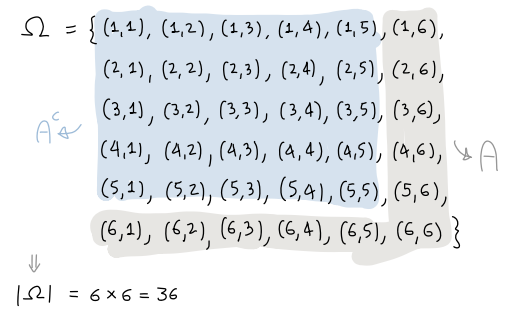
\includegraphics[width=.7\textwidth]{images/almeno_uno.png}
    \end{center}
    \paragraph{Soluzioni}
    Contando gli elementi abbiamo due possibili soluzioni:
    \begin{enumerate}
        \item $|A|=11\implies P(A) = \frac{|A|}{|\Omega|} = \frac{11}{36}$
        \item $A^c= $"Non esce neanche un 6$ = \{1,2,3,4,5\} \times \{1,2,3,4,5\}$.
        $|A^c|= 5 \times 5 = 25 $.
        \\ $P(A^c) = \frac{|A^c|}{|\Omega|} = \frac{25}{36} \implies P(A) = 1 - P(A^c) = \frac{11}{36}$
    \end{enumerate}
 }


\pagebreak
\section{Calcolo combinatorio}
Consideriamo uno spazio di Probabilità Uniforme, in cui $P(A) = \frac{|A|}{|\Omega|}$.
In questo tipo di spazio calcolare una probabilità significa \textbf{contare gli elementi di un insieme}.

Dato che contare non è banale per insiemi grandi sono nate tecniche di conteggio,
esse formano il \textbf{Calcolo Combinatorio}
\definizione{
\textbf{Principio Fondamentale}:
Consideriamo un esperimento costituito da due parti:
\begin{enumerate}
    \item Prima parte con $n$ esiti possibili $\{a_1,...,a_n\}$.
    \item Seconda parte con $m$ esiti possibili  $\{b_1,...,b_m\}$.
\end{enumerate}
L'esperimento totale può avere \textbf{$n\cdot m$ esiti possibili}.
\[ \Omega = \{ (a_i,b_j) : 1\leq i \leq n, 1 \leq j \leq n\} \implies |\Omega|= n \cdot m \]
}
Abbiamo visto l'esempio del lancio di due dadi a sei facce, in cui:
  \[ \Omega=\{(x,y): x,y \in \{1,2,3,4,5,6\}\} \implies |\Omega| = 6\cdot6 = 36 \]
Se lanciassi tre dadi $|\Omega| = 6\cdot6\cdot 6 = 216$ esiti possibili e così via.

\subsection{Disposizioni con ripetizione}
Le disposizioni con ripetizione possono essere definite come segue:
\definizione{
    \textbf{Disposizioni con Ripetizione}:
    Sequenze ordinate di $k$ elementi (anche ripetuti) scelti tra $n$ possibili.
    Il numero totale è:
    \begin{equation}
        n*n \dots n = n^k
    \end{equation}
}

\esempio{
    Estraggo casualmente 3 persone: Qual'è la probabilità che siano tutte nate in primavera?
    In questo caso lo \textbf{Spazio Campionario} sono i compleanni delle tre persone, quindi:
    \[
        \Omega = \{(x_1, x_2, x_3): x_1, x_2, x_3 \in \text{ Calendario}\}
    \]
    Questa è una disposizione con ripetizione di 3 elementi estratti dal calendario.
    \[
        |\Omega| = 365*365*365 = 365^3
    \]
    Abbiamo una \textbf{Probabilità Uniforme}: $P(A) = \frac{|A|}{|\Omega|}$
    \\Troviamo $|A|$: Consideriamo tutte le persone nate tra il 20 marzo e il 21 giugno:
    \begin{center}
        A = "tutti nati in primavera" = [20 marzo, 21 giugno) $\to$ 92 giorni
    \end{center}
    Si tratta anche qua di una disposizione con ripetizione di 3 elementi.
    \[
        |A| = 92*92*92 = 92^3 (= 778.688)
    \]
    Per calcolare la probabilità è sufficiente dividere $A$ per $\Omega$
    \[
        P(A) = \frac{|A|}{|\Omega|} = \frac{92^3}{365^3} = 0,016 = 1,6\%
    \]
    Se avessi estratto k persone sarebbe stato sufficiente sostituire l'esponente con k.
}

\osservazione{
    Esperimenti molto diversi, come lanciare 3 dadi o estrarre 3 persone e osservarne i compleanni,
     ammettono la \textbf{Stessa descrizione matematica}:
     \[
        \Omega = \{(x_1, x_2, x_3): x_1, x_2, x_3 \in E\}
    \]
    \[
        \Omega = \{\text {Disposizione con Ripetizione di tre elementi estratti da E}\}
    \]
    Con $E = \{1,2,3,4,5,6\}$ oppure $E = \text{ Calendario}$, in ogni caso avremo sempre che $|\Omega| = |E|^3$. 
}

\subsection{Disposizioni semplici}
Ora chiediamoci: Quanti sono gli esiti del lancio di due dadi i cui numeri ottenuti sono \textbf{distinti}?
\\Quante coppie $(x,y)$ con $x\neq y$, se $x,y \in \{1,2,3,4,5,6\}$?

\definizione{
    \textbf{Disposizioni Semplici}\footnote{Semplici si intende "Senza Ripetizione"}:
    Sequenze ordinate di $k$ elementi distinti scelti tra $n$ possibili (con $k <= n$).
    Sono in numero:
    \begin{equation}
        n*(n-1)*(n-2)\dots(n-k+1) = \frac{n!}{(n-k)!}
    \end{equation}
}
\nb{E preferibile utilizzare la prima formula su R dato che il fattoriale scala molto male,
su carta spesso si semplifica, ma su Computer si calcolerebbe tutto il fattoriale e spesso richiede 
molto tempo.}
Un caso speciale è se $k = n$: in questo caso si parla di \textbf{Permutazioni} di $n$ oggetti. 
Sono in numero:
\begin{equation}
    n! = n*(n-1)*(n-2)\dots 2 * 1
\end{equation}

\esempio{
Quanti sono i possibili ordini di arrivo di 3 squadre, $a$, $b$ e $c$?
\\Si tratta di una \textbf{permutazione} di 3 elementi:
\[ abc,acb,bac,bca,cab,cba \]
E sono esattamente $3! = 3\cdot 2 \cdot 1$
}
%\esempio{Paradosso dei compleanni}

\subsection{Combinazioni}
In molti casi non siamo interessati all'ordine. 
Per esempio, se dobbiamo scegliere un comitato di 2 persone non ci interessa l'ordine 
dei candidati.
Si parla in questo caso di \textbf{combinazioni}, esse si possono ottenere dalle disposizioni semplici
"dimenticando" l'ordine degli elementi.

\definizione{
    \textbf{Combinazioni}: Insiemi = Collezioni
    \begin{equation}
        {n \choose x} = \frac{n!}{k!(n-k)!}
    \end{equation}
}

Insiemi = collezioni (non ordinate) di k elementi distinti scelti tra n possibili (con $k <= n$).
\paragraph{Esempio}. Mano di carte a Poker, un giocatore riceve 5 carte estratte da un mazzo che
ne contiene 52. Il numero di possibili mani è
\begin{equation}
    {52 \choose 5} = \frac{52!}{5!47!}
\end{equation} 

\section{Probabilità Condizionata}
Consideriamo un esperimento aleatorio, che descriviamo con uno spazio di probabilità $(\Omega, P)$.
Consideriamo un evento $A \subseteq \Omega$, che ha un probabilità $P(A)$.
Supponiamo di ricevere l'informazione che un altro evento B si è verificato.
Come è ragionevole aggiornare la probabilità di A per tenere conto di questa informazione aggiuntiva?
\\La soluzione è data dalla probabilità Condizionata.
\begin{equation}
    P(A|B) = \frac{P(A \cap B)}{P(B)}
\end{equation}
La precedente formula denota la probabilità condizionata di A dato B (o sapendo B).
Sto quindi calcolando la probabilità di A.
\begin{center}
    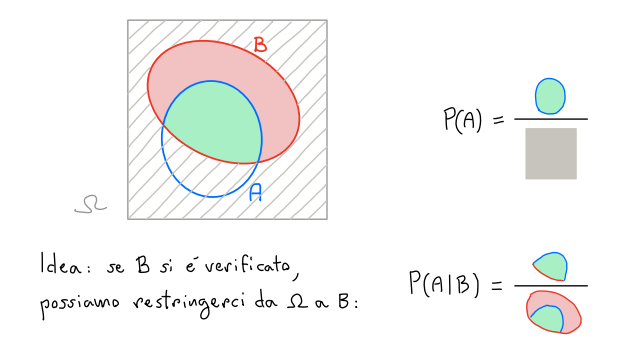
\includegraphics[width=120mm,scale=0.5]{prob_condizionata_area.png}    
\end{center}
Quando si verifica un evento lo spazio di probabilità si riduce (vedere esempio sui dadi)
\subsection{Regola del prodotto}
\begin{equation}
    P(A \cap B) = P(A)*P(B|A)
\end{equation}
\subsection{Formula di Disintegrazione}
\begin{equation}
    P(A) = P(A \cap B) + P(A \cap B^c)
\end{equation}
\subsection{Formula delle probabilità totali}
\begin{equation}
    P(A) = P(A|B)P(B) + P(A|B^c)P(B^c)
\end{equation}
Inoltre $P(*|B)$ + una probabilità, in particolare:
\begin{equation}
    P(A^c|B) = 1 - P(A|B)
\end{equation}
\subsection{Formula di Bayes}
\begin{equation}
    P(B|A) = \frac{P(A|B)P(B)}{P(A)}
\end{equation}
\paragraph{Esempio}. Per vedere la parte pratica andare a vedere l'esempio sui tamponi
per rilveare la presenza di un virus. Super interessante e utile.
\\Il file è \textbf{Appunti Lezione 3 - In fondo al PDF}

\section{Indipendenza di eventi}
Può capitare che, per un evento A, l'informazione che un altro evento B si è verificato
non ne cambi la probabilità.
\begin{equation}
    P(A|B) = P(A)
\end{equation}
che equivale
\begin{equation}
    P(A \cap B) = P(A)P(B)
\end{equation}
In questo caso gli eventi A e B si dicono \textbf{Indipendenti}
\paragraph{Esempi}
Lancio di due dadi, i risultati sono eventi indipendenti
\\ Urna contenente 5 palline rosse e 3 palline verdi. Pesco in successione due palline, 
senza reimmissione. La probabilità che la prima pallina sia rossa e che la seconda sia rossa
sono \textbf{dipendenti}!

\subsection{Eventi indipendenti != Eventi disgiunti!}
\begin{center}
    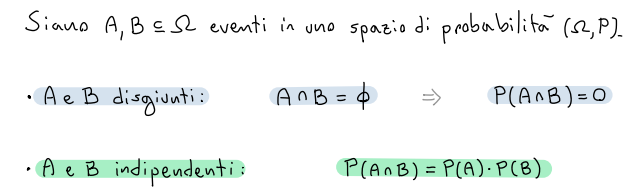
\includegraphics[width=120mm, scale=0.5]{differenza_disgiunti_indipendenti.png}
\end{center}
Quindi due eventi indipendenti non possono essere disgiunti,
tranne nel caso "banale" in cui uno dei due abbia probabilità
nulla.

\paragraph*{Esempio} Una famiglia ha due figli/e descritti da 
\\ $\Omega = \{MM, FF, FM, FF\}$ e $P=\text{Probabilità uniforme} = \frac{1}{4}$
\\ Consideriamo gli eventi:
\begin{itemize}
    \item A := "il primo genito è maschio" = \{MM, FF\}
    \item B := "il secondo genito è maschio" = \{MM, FM\}
    \item C := "la primogenita è femmina" =\{FM, FF\}
\end{itemize}
\begin{center}
    In questo caso A e B sono \textbf{indipendenti}, ma \textbf{NON disgiunti};
\\ A e C sono \textbf{disgiunti}, ma \textbf{NON indipendenti}.
\end{center}

\paragraph{Estensioni}
Tre eventi A, B, C si dicono indipendenti se valgono
\begin{center}
    $P(A \cap B \cap C) = P(A)P(B)P(C)$
    \\$P(A \cap B) = P(A)P(B)$
    \\$P(B \cap C) = P(B)P(C)$
    \\$P(A \cap C) = P(A)P(C)$
\end{center}
